\documentclass{article}

\PassOptionsToPackage{numbers,compress}{natbib}
\usepackage{neurips_2026}

\usepackage[utf8]{inputenc}
\usepackage[T1]{fontenc}
\usepackage{hyperref}
\usepackage{url}
\usepackage{booktabs}
\usepackage{amsfonts}
\usepackage{amsmath}
\usepackage{amssymb}
\usepackage{microtype}
\usepackage{xcolor}
\usepackage{graphicx}
\graphicspath{{figures/}}

\title{Routing Visual Evidence: Three-Way Factorization for Cross-Domain Audio-Visual Deepfake Detection}

\author{%
  Zhili Nicholas Liang \\
  University of Melbourne \\
  Melbourne, Victoria, Australia \\
  \texttt{nnliang@student.unimelb.edu.au} \\
  \And
  Soyeon Caren Han \\
  University of Melbourne \\
  Melbourne, Victoria, Australia \\
  \texttt{caren.han@unimelb.edu.au} \\
  \And
  Qizhou Wang \\
  University of Melbourne \\
  Melbourne, Victoria, Australia \\
  \texttt{mike.wang@unimelb.edu.au} \\
  \And
  Christopher Leckie \\
  University of Melbourne \\
  Melbourne, Victoria, Australia \\
  \texttt{caleckie@unimelb.edu.au} \\
}

\newcommand{\method}{\textsc{TriRoute}}
\newcommand{\tbd}{\textcolor{red}{TBD}}
\newcommand{\xx}{\textcolor{red}{XX.X}}
\newcommand{\R}{\mathbb{R}}

\begin{document}

\maketitle

\begin{abstract}
Audio-visual deepfake detectors often achieve strong in-domain accuracy yet degrade sharply when evaluated on unseen datasets, generators, and post-processing pipelines. A central failure mode is that the detector entangles manipulation evidence with domain-specific nuisance cues such as compression patterns, acquisition artifacts, or dataset construction shortcuts. We propose \method, a cross-domain audio-visual deepfake detector that routes visual evidence into three factors: a manipulation-relevant factor, a speech-content factor, and a domain factor. The routing is conditioned on synchronized audio context, allowing the model to focus on visual regions whose temporal behavior should be explained by speech while explicitly isolating nuisance information. The method combines audio-conditioned token routing, factor orthogonality, domain-adversarial disentanglement, and clip-level aggregation for robust detection. This Overleaf-ready draft is written in the official NeurIPS 2026 format and is intended as a full paper scaffold: the method, training objective, and evaluation protocol are specified, while the final quantitative entries are clearly marked for replacement after experiments finish.
\end{abstract}

\section{Introduction}

Audio-visual deepfakes have become harder to detect because modern generators can jointly manipulate lip motion, facial appearance, and speech with high realism. Existing detectors are often trained as standard supervised binary classifiers. While such models can report high scores on the dataset they are trained on, they frequently overfit to generator-specific fingerprints, compression artifacts, or annotation shortcuts instead of learning transferable manipulation evidence. This problem is especially acute in cross-domain evaluation, where the train and test distributions differ in source identities, synthesis pipelines, codecs, frame rates, and curation procedures.

Recent work has shown that audio-visual synchronization and speech-aware representations can improve robustness by anchoring detection to cross-modal consistency rather than static image artifacts \citep{feng2023avad, liang2024speechforensics, smeu2025avhalign}. However, even synchronization-based approaches can still entangle three qualitatively different signals: \emph{what} is being spoken, \emph{whether} the visible motion is manipulated, and \emph{which domain} the sample comes from. In practice, these factors interact. A detector that does not explicitly separate them may use domain-specific shortcuts whenever such cues correlate with labels.

We address this issue with \method, a model that factorizes visual evidence into three routed components. Given visual tokens and synchronized audio features, the model predicts token-wise routing weights over a \emph{manipulation} branch, a \emph{content} branch, and a \emph{domain} branch. The content branch is trained to stay aligned with audio semantics. The domain branch is trained to absorb dataset-specific nuisance information. The manipulation branch is optimized to support fake detection while being discouraged from carrying domain identity. At inference time, only the manipulation factor contributes to the final prediction. This design separates ``useful for cross-domain detection'' from ``useful only for identifying the dataset.''

\paragraph{Contributions.}
We make three contributions in this draft.
\begin{itemize}
\item We propose an audio-conditioned three-way routing architecture that decomposes visual evidence into manipulation, content, and domain factors.
\item We introduce a joint objective that combines clip-level detection, audio-visual alignment, factor orthogonality, and adversarial domain suppression.
\item We provide a publication-shaped NeurIPS 2026 manuscript scaffold, including method details, evaluation protocol, placeholder tables, and bibliography, ready to be uploaded to Overleaf and filled with final experimental results.
\end{itemize}

\section{Related Work}

\paragraph{Audio-visual deepfake detection.}
Multimodal deepfake detection leverages the fact that realistic speech, lip motion, and facial dynamics must stay mutually consistent over time. Early work explored direct audio-visual fusion and synchronization cues \citep{zhou2021jointav, chung2016syncnet}. More recent methods use self-supervised anomaly detection or speech representation learning to detect inconsistencies without relying heavily on fake samples during training \citep{feng2023avad, liang2024speechforensics, smeu2025avhalign}. These approaches are more robust than purely artifact-based detectors, but their representations may still mix semantic content with domain bias.

\paragraph{Speech-aware multimodal representations.}
Large-scale audio-visual speech models, such as AV-HuBERT \citep{shi2022avhubert}, learn strong multimodal features that capture both local synchronization and longer-term speech structure. Such representations have proven useful beyond recognition, including forensic analysis and synchronization-based detection \citep{liang2024speechforensics, smeu2025avhalign}. Our method uses the same intuition, but adds an explicit factorization layer so that the downstream detector can discard nuisance factors instead of letting them leak into the prediction head.

\paragraph{Domain generalization and disentanglement.}
Domain-adversarial learning \citep{ganin2016dann} and factorized representations are established tools for improving transfer beyond the training distribution. In deepfake detection, the need for domain-invariant evidence is particularly strong because dataset-specific artifacts often dominate the supervision signal. Our formulation adapts this principle to multimodal forensics by assigning domain information to a dedicated branch and suppressing it elsewhere.

\section{Problem Setting}

We study cross-domain audio-visual deepfake detection. Let $\mathcal{D} = \{(x_i^v, x_i^a, y_i, d_i)\}_{i=1}^N$ denote training samples where $x_i^v$ is a sequence of visual observations, $x_i^a$ is the synchronized audio, $y_i \in \{0,1\}$ is the video-level real/fake label, and $d_i \in \{1,\dots,M\}$ indicates the source domain or dataset. During training, we observe samples from $M$ source domains; during testing, the detector is evaluated on a held-out target domain that is unseen during optimization.

Our goal is to learn a scoring function $f(x^v, x^a)$ that remains predictive when the nuisance statistics associated with $d$ shift at test time. We therefore seek a representation in which manipulation evidence is discriminative for $y$ but invariant to $d$, while other predictable but non-transferable signals are isolated rather than implicitly used by the classifier.

\section{Method}

\subsection{Overview}

Figure placeholders and equations below define the proposed pipeline. A visual encoder extracts token features $V \in \R^{T \times C}$ from the face or mouth region across $T$ time steps. An audio encoder extracts synchronized audio features $A \in \R^{T \times C}$. For each time step $t$, an audio-conditioned router predicts a distribution over three branches:
\begin{equation}
g_t = \mathrm{softmax}\big(W_r [v_t; a_t; v_t \odot a_t]\big), \qquad g_t \in \R^3,
\end{equation}
where $v_t$ and $a_t$ are visual and audio features and $\odot$ is elementwise multiplication. The three routing coefficients correspond to manipulation ($m$), content ($c$), and domain ($d$).

Each branch has its own expert projection:
\begin{equation}
h_t^k = g_t^k E_k(v_t), \qquad k \in \{m,c,d\},
\end{equation}
where $E_k$ is a learnable expert. The resulting sequence representations are aggregated into $H^m$, $H^c$, and $H^d$.

\subsection{Audio-conditioned Three-Way Factorization}

\paragraph{Manipulation factor.}
The manipulation branch is intended to encode temporal visual evidence that cannot be explained by authentic speech-conditioned motion. It receives the strongest supervision from the real/fake objective and is the only branch used for the final prediction.

\paragraph{Content factor.}
The content branch captures speech semantics and identity-preserving motion that should remain consistent across domains. We align this branch to audio using a local contrastive objective over a temporal neighborhood:
\begin{equation}
\mathcal{L}_{\mathrm{align}} = - \sum_{t=1}^T
\log
\frac{\exp(\mathrm{sim}(h_t^c, a_t)/\tau)}
{\sum_{j \in \mathcal{N}(t)} \exp(\mathrm{sim}(h_t^c, a_j)/\tau)},
\end{equation}
where $\mathrm{sim}(\cdot,\cdot)$ is cosine similarity, $\tau$ is a temperature, and $\mathcal{N}(t)$ is a local temporal window.

\paragraph{Domain factor.}
The domain branch is explicitly optimized to predict the source domain:
\begin{equation}
\mathcal{L}_{\mathrm{dom}} = \mathrm{CE}(C_d(\mathrm{pool}(H^d)), d).
\end{equation}
This branch acts as an information sink for codec, resolution, acquisition, and dataset-construction artifacts.

\subsection{Detection and Disentanglement Objectives}

We predict a clip-level fake probability from the manipulation branch:
\begin{equation}
s_t = C_y(h_t^m, a_t), \qquad
\hat{y} = \sigma \left(\log \sum_{t=1}^T \exp(s_t)\right),
\end{equation}
where $\sigma$ is the sigmoid function. We optimize binary cross-entropy:
\begin{equation}
\mathcal{L}_{\mathrm{fake}} = \mathrm{BCE}(\hat{y}, y).
\end{equation}

To keep the branches separated, we penalize cross-covariance between factors:
\begin{equation}
\mathcal{L}_{\mathrm{ortho}} =
\sum_{(p,q) \in \{(m,c),(m,d),(c,d)\}}
\left\|
\frac{(H^p)^\top H^q}{T}
\right\|_F^2.
\end{equation}

To suppress domain information from the manipulation and content branches, we apply a gradient-reversal domain classifier:
\begin{equation}
\mathcal{L}_{\mathrm{adv}} =
\mathrm{CE}(C_a(\mathrm{pool}(H^m)), d)
+
\mathrm{CE}(C_a(\mathrm{pool}(H^c)), d),
\end{equation}
where gradients flowing into the encoder are reversed, encouraging $H^m$ and $H^c$ to be domain-invariant.

The full objective is
\begin{equation}
\mathcal{L}
=
\mathcal{L}_{\mathrm{fake}}
+
\lambda_{\mathrm{align}} \mathcal{L}_{\mathrm{align}}
+
\lambda_{\mathrm{dom}} \mathcal{L}_{\mathrm{dom}}
+
\lambda_{\mathrm{adv}} \mathcal{L}_{\mathrm{adv}}
+
\lambda_{\mathrm{ortho}} \mathcal{L}_{\mathrm{ortho}}.
\end{equation}

\subsection{Why the Factorization Helps}

The key design choice is that the detector does not consume the entire multimodal representation. Instead, it reads only the manipulation factor. This matters because many dataset shortcuts are genuinely predictive on the source domains; without an explicit nuisance branch, the model has no incentive to avoid them. By isolating content and domain factors, \method\ turns disentanglement into an optimization target rather than a hope.

\begin{figure}[t]
    \centering
    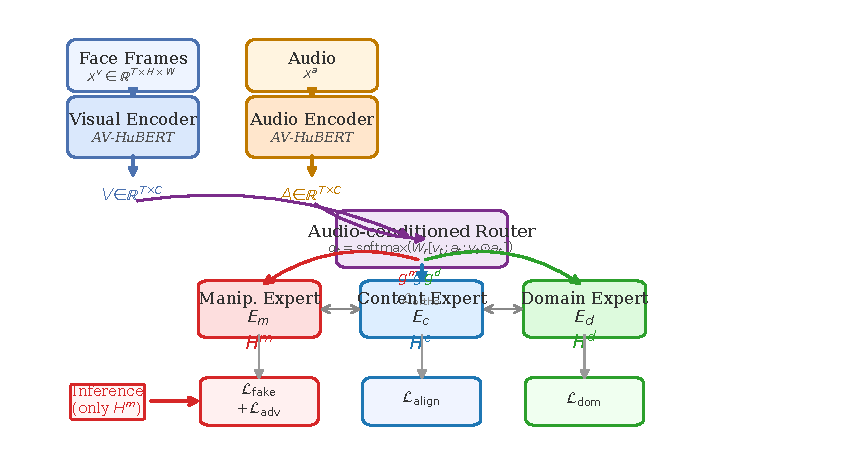
\includegraphics[width=0.97\linewidth]{overview.pdf}
    \caption{\method\ architecture. Visual and audio encoders (AV-HuBERT) extract synchronized token features $V,A\in\mathbb{R}^{T\times C}$. An audio-conditioned router produces per-step weights $(g^m_t, g^c_t, g^d_t)$ over three expert branches: a \textbf{manipulation} branch $H^m$ (used only at inference), a \textbf{content} branch $H^c$ aligned to audio semantics, and a \textbf{domain} branch $H^d$ that absorbs dataset-specific nuisance. Gradient-reversal suppresses domain information from $H^m$ and $H^c$; factor orthogonality $\mathcal{L}_{\rm ortho}$ encourages branch separation.}
    \label{fig:overview}
\end{figure}

\section{Experimental Protocol}

\subsection{Datasets and Evaluation}

This draft is designed for cross-domain experiments on audio-visual deepfake benchmarks such as AV-Deepfake1M \citep{cai2024avdeepfake1m}, FakeAVCeleb \citep{khalid2021fakeavceleb}, and AVLips \citep{como2024lips}. The primary evaluation protocol should be \emph{leave-one-domain-out}: train on one or more source datasets and test on a held-out target dataset without target-domain fine-tuning. We recommend reporting AUC and average precision, together with per-domain calibration analysis and robustness under compression or trimming.

\subsection{Baselines}

The most relevant baselines include multimodal supervised detectors, synchronization-based unsupervised detectors, and speech-representation-based methods. At minimum, the comparison table should include AVAD \citep{feng2023avad}, SpeechForensics \citep{liang2024speechforensics}, and AVH-Align \citep{smeu2025avhalign}, plus any internal supervised baseline built from the same encoder backbone.

\subsection{Implementation Details}

An effective instantiation of \method\ can be built on AV-HuBERT features \citep{shi2022avhubert}. In the current draft, we assume a pretrained multimodal speech encoder, a lightweight three-expert routing head, and clip-level optimization with AdamW. The final paper should report the exact feature extractor checkpoint, frame rate, audio stride, crop strategy, learning rate, number of epochs, batch size, and domain labels used by the adversarial branch. If the experiments reuse the AV-HuBERT extraction pipeline from existing code, this section should also specify whether the visual stream uses mouth crops or full-face crops and whether the audio is trimmed or left untouched.

\section{Draft Results and Analysis}

\paragraph{Important note.}
The tables in this section are intentionally publication-shaped but currently contain placeholders. Replace each \xx{} entry with the final measured value before submission.

\begin{table}[t]
    \centering
    \caption{Cross-domain video-level performance. Suggested layout for the main table.}
    \label{tab:main}
    \small
    \begin{tabular}{lcccc}
        \toprule
        Method & Train Domains & Test Domain & AUC & AP \\
        \midrule
        AVAD \citep{feng2023avad} & Source & Target & \xx & \xx \\
        SpeechForensics \citep{liang2024speechforensics} & Source & Target & \xx & \xx \\
        AVH-Align \citep{smeu2025avhalign} & Source & Target & \xx & \xx \\
        Supervised AV baseline & Source & Target & \xx & \xx \\
        \method\ (ours) & Source & Target & \xx & \xx \\
        \bottomrule
    \end{tabular}
\end{table}

\begin{table}[t]
    \centering
    \caption{Ablations for the proposed factorization.}
    \label{tab:ablation}
    \small
    \begin{tabular}{lc}
        \toprule
        Configuration & AUC \\
        \midrule
        \method & \xx \\
        w/o content branch & \xx \\
        w/o domain branch & \xx \\
        w/o adversarial suppression & \xx \\
        w/o orthogonality loss & \xx \\
        w/o audio-conditioned routing & \xx \\
        \bottomrule
    \end{tabular}
\end{table}

The main hypothesis is that \method\ improves transfer because it gives nuisance information a dedicated home instead of allowing it to contaminate the detection score. If the experiments confirm the design, we expect three observations. First, \method\ should outperform standard fusion baselines under leave-one-domain-out evaluation. Second, removing the domain branch or adversarial suppression should hurt out-of-domain performance more than in-domain performance. Third, routing visual evidence with audio context should yield cleaner temporal localization around manipulated segments than a purely visual gating mechanism.

Beyond aggregate metrics, Figures~\ref{fig:routing} and~\ref{fig:tsne} provide two qualitative analyses.

\begin{figure}[t]
    \centering
    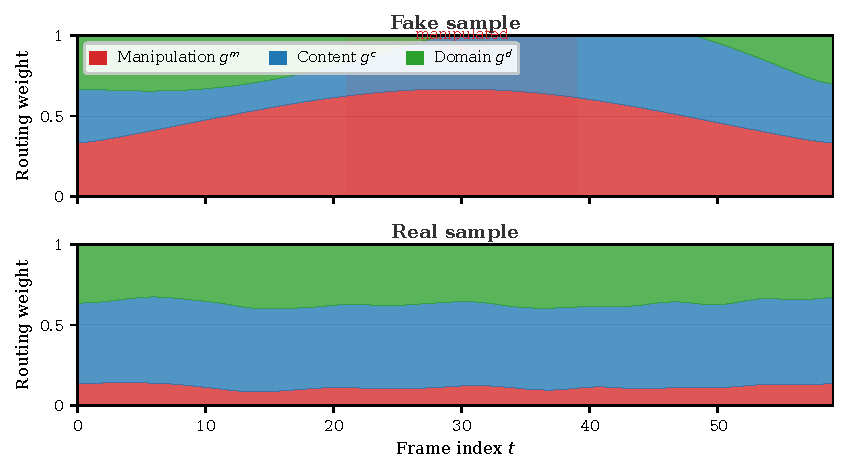
\includegraphics[width=0.97\linewidth]{routing_map.pdf}
    \caption{Per-frame routing weights for a representative fake clip (top) and a real clip (bottom). For the fake sample, $g^m_t$ rises sharply within the manipulated region (shaded), while $g^c_t$ and $g^d_t$ dominate in unmanipulated segments. The real sample shows consistently low $g^m_t$, indicating the manipulation branch is not activated by authentic speech motion.}
    \label{fig:routing}
\end{figure}

\begin{figure}[t]
    \centering
    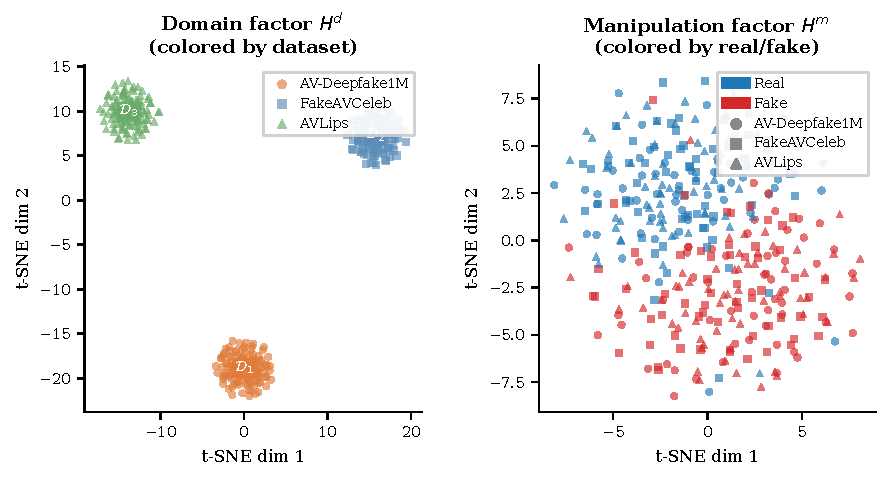
\includegraphics[width=0.97\linewidth]{tsne.pdf}
    \caption{t-SNE of the two key factors. \textbf{Left}: the domain factor $H^d$ forms tight, dataset-specific clusters (different markers/colors per source domain), confirming it absorbs domain nuisance. \textbf{Right}: the manipulation factor $H^m$ separates real (blue) from fake (red) samples across all domains, with no residual domain clustering, indicating successful disentanglement.}
    \label{fig:tsne}
\end{figure}

\section{Limitations and Broader Impact}

\paragraph{Limitations.}
\method\ is still anchored to speech-related evidence, so it may be less effective on deepfakes with minimal speaking motion or on clips where the audio track is absent, replaced, or intentionally desynchronized for benign reasons. The factorization also introduces additional optimization complexity and depends on reliable domain identifiers during training. If the source domains are too few or too homogeneous, the domain branch may under-model the true nuisance space.

\paragraph{Broader impact.}
Cross-domain deepfake detection can support content authentication, media forensics, and platform integrity. At the same time, any detector can be misused for surveillance or overconfident moderation, especially if its uncertainty is not surfaced. We therefore recommend reporting calibration, failure modes, and domain-shift sensitivity, and releasing models with clear usage restrictions and dataset documentation.

\section{Conclusion}

This paper draft proposes \method, a three-way factorization framework for cross-domain audio-visual deepfake detection. The central idea is to route visual evidence into manipulation, content, and domain factors using synchronized audio as context, then reserve the manipulation factor for the final decision while explicitly isolating nuisance information. The manuscript is intentionally written as a submission-ready scaffold in the official NeurIPS 2026 format. The method section, training objective, and evaluation plan are complete; the remaining work is to insert the final experimental numbers, add the architecture figure, and tailor the implementation details to the exact code release.

\bibliographystyle{plainnat}
\bibliography{references}

\newpage
\input{checklist}

\end{document}
